\documentclass[conference]{IEEEtran}

% *** MISC UTILITY PACKAGES ***
%
%\usepackage{ifpdf}
% Heiko Oberdiek's ifpdf.sty is very useful if you need conditional
% compilation based on whether the output is pdf or dvi.
% usage:
% \ifpdf
%   % pdf code
% \else
%   % dvi code
% \fi
% The latest version of ifpdf.sty can be obtained from:
% http://www.ctan.org/tex-archive/macros/latex/contrib/oberdiek/
% Also, note that IEEEtran.cls V1.7 and later provides a builtin
% \ifCLASSINFOpdf conditional that works the same way.
% When switching from latex to pdflatex and vice-versa, the compiler may
% have to be run twice to clear warning/error messages.






% *** CITATION PACKAGES ***
%
%\usepackage{cite}
% cite.sty was written by Donald Arseneau
% V1.6 and later of IEEEtran pre-defines the format of the cite.sty package
% \cite{} output to follow that of IEEE. Loading the cite package will
% result in citation numbers being automatically sorted and properly
% "compressed/ranged". e.g., [1], [9], [2], [7], [5], [6] without using
% cite.sty will become [1], [2], [5]--[7], [9] using cite.sty. cite.sty's
% \cite will automatically add leading space, if needed. Use cite.sty's
% noadjust option (cite.sty V3.8 and later) if you want to turn this off.
% cite.sty is already installed on most LaTeX systems. Be sure and use
% version 4.0 (2003-05-27) and later if using hyperref.sty. cite.sty does
% not currently provide for hyperlinked citations.
% The latest version can be obtained at:
% http://www.ctan.org/tex-archive/macros/latex/contrib/cite/
% The documentation is contained in the cite.sty file itself.






% *** GRAPHICS RELATED PACKAGES ***
%
\ifCLASSINFOpdf
  \usepackage[pdftex]{graphicx}
  % declare the path(s) where your graphic files are
  % \graphicspath{{../pdf/}{../jpeg/}}
  % and their extensions so you won't have to specify these with
  % every instance of \includegraphics
  % \DeclareGraphicsExtensions{.pdf,.jpeg,.png}
\else
  % or other class option (dvipsone, dvipdf, if not using dvips). graphicx
  % will default to the driver specified in the system graphics.cfg if no
  % driver is specified.
  % \usepackage[dvips]{graphicx}
  % declare the path(s) where your graphic files are
  % \graphicspath{{../eps/}}
  % and their extensions so you won't have to specify these with
  % every instance of \includegraphics
  % \DeclareGraphicsExtensions{.eps}
\fi
% graphicx was written by David Carlisle and Sebastian Rahtz. It is
% required if you want graphics, photos, etc. graphicx.sty is already
% installed on most LaTeX systems. The latest version and documentation can
% be obtained at:
% http://www.ctan.org/tex-archive/macros/latex/required/graphics/
% Another good source of documentation is "Using Imported Graphics in
% LaTeX2e" by Keith Reckdahl which can be found as epslatex.ps or
% epslatex.pdf at: http://www.ctan.org/tex-archive/info/
%
% latex, and pdflatex in dvi mode, support graphics in encapsulated
% postscript (.eps) format. pdflatex in pdf mode supports graphics
% in .pdf, .jpeg, .png and .mps (metapost) formats. Users should ensure
% that all non-photo figures use a vector format (.eps, .pdf, .mps) and
% not a bitmapped formats (.jpeg, .png). IEEE frowns on bitmapped formats
% which can result in "jaggedy"/blurry rendering of lines and letters as
% well as large increases in file sizes.
%
% You can find documentation about the pdfTeX application at:
% http://www.tug.org/applications/pdftex





% *** MATH PACKAGES ***
%
%\usepackage[cmex10]{amsmath}
% A popular package from the American Mathematical Society that provides
% many useful and powerful commands for dealing with mathematics. If using
% it, be sure to load this package with the cmex10 option to ensure that
% only type 1 fonts will utilized at all point sizes. Without this option,
% it is possible that some math symbols, particularly those within
% footnotes, will be rendered in bitmap form which will result in a
% document that can not be IEEE Xplore compliant!
%
% Also, note that the amsmath package sets \interdisplaylinepenalty to 10000
% thus preventing page breaks from occurring within multiline equations. Use:
%\interdisplaylinepenalty=2500
% after loading amsmath to restore such page breaks as IEEEtran.cls normally
% does. amsmath.sty is already installed on most LaTeX systems. The latest
% version and documentation can be obtained at:
% http://www.ctan.org/tex-archive/macros/latex/required/amslatex/math/





% *** SPECIALIZED LIST PACKAGES ***
%
%\usepackage{algorithmic}
% algorithmic.sty was written by Peter Williams and Rogerio Brito.
% This package provides an algorithmic environment fo describing algorithms.
% You can use the algorithmic environment in-text or within a figure
% environment to provide for a floating algorithm. Do NOT use the algorithm
% floating environment provided by algorithm.sty (by the same authors) or
% algorithm2e.sty (by Christophe Fiorio) as IEEE does not use dedicated
% algorithm float types and packages that provide these will not provide
% correct IEEE style captions. The latest version and documentation of
% algorithmic.sty can be obtained at:
% http://www.ctan.org/tex-archive/macros/latex/contrib/algorithms/
% There is also a support site at:
% http://algorithms.berlios.de/index.html
% Also of interest may be the (relatively newer and more customizable)
% algorithmicx.sty package by Szasz Janos:
% http://www.ctan.org/tex-archive/macros/latex/contrib/algorithmicx/




% *** ALIGNMENT PACKAGES ***
%
%\usepackage{array}
% Frank Mittelbach's and David Carlisle's array.sty patches and improves
% the standard LaTeX2e array and tabular environments to provide better
% appearance and additional user controls. As the default LaTeX2e table
% generation code is lacking to the point of almost being broken with
% respect to the quality of the end results, all users are strongly
% advised to use an enhanced (at the very least that provided by array.sty)
% set of table tools. array.sty is already installed on most systems. The
% latest version and documentation can be obtained at:
% http://www.ctan.org/tex-archive/macros/latex/required/tools/


%\usepackage{mdwmath}
%\usepackage{mdwtab}
% Also highly recommended is Mark Wooding's extremely powerful MDW tools,
% especially mdwmath.sty and mdwtab.sty which are used to format equations
% and tables, respectively. The MDWtools set is already installed on most
% LaTeX systems. The lastest version and documentation is available at:
% http://www.ctan.org/tex-archive/macros/latex/contrib/mdwtools/


% IEEEtran contains the IEEEeqnarray family of commands that can be used to
% generate multiline equations as well as matrices, tables, etc., of high
% quality.


%\usepackage{eqparbox}
% Also of notable interest is Scott Pakin's eqparbox package for creating
% (automatically sized) equal width boxes - aka "natural width parboxes".
% Available at:
% http://www.ctan.org/tex-archive/macros/latex/contrib/eqparbox/





% *** SUBFIGURE PACKAGES ***
%\usepackage[tight,footnotesize]{subfigure}
% subfigure.sty was written by Steven Douglas Cochran. This package makes it
% easy to put subfigures in your figures. e.g., "Figure 1a and 1b". For IEEE
% work, it is a good idea to load it with the tight package option to reduce
% the amount of white space around the subfigures. subfigure.sty is already
% installed on most LaTeX systems. The latest version and documentation can
% be obtained at:
% http://www.ctan.org/tex-archive/obsolete/macros/latex/contrib/subfigure/
% subfigure.sty has been superceeded by subfig.sty.



%\usepackage[caption=false]{caption}
%\usepackage[font=footnotesize]{subfig}
% subfig.sty, also written by Steven Douglas Cochran, is the modern
% replacement for subfigure.sty. However, subfig.sty requires and
% automatically loads Axel Sommerfeldt's caption.sty which will override
% IEEEtran.cls handling of captions and this will result in nonIEEE style
% figure/table captions. To prevent this problem, be sure and preload
% caption.sty with its "caption=false" package option. This is will preserve
% IEEEtran.cls handing of captions. Version 1.3 (2005/06/28) and later
% (recommended due to many improvements over 1.2) of subfig.sty supports
% the caption=false option directly:
%\usepackage[caption=false,font=footnotesize]{subfig}
%
% The latest version and documentation can be obtained at:
% http://www.ctan.org/tex-archive/macros/latex/contrib/subfig/
% The latest version and documentation of caption.sty can be obtained at:
% http://www.ctan.org/tex-archive/macros/latex/contrib/caption/




% *** FLOAT PACKAGES ***
%
%\usepackage{fixltx2e}
% fixltx2e, the successor to the earlier fix2col.sty, was written by
% Frank Mittelbach and David Carlisle. This package corrects a few problems
% in the LaTeX2e kernel, the most notable of which is that in current
% LaTeX2e releases, the ordering of single and double column floats is not
% guaranteed to be preserved. Thus, an unpatched LaTeX2e can allow a
% single column figure to be placed prior to an earlier double column
% figure. The latest version and documentation can be found at:
% http://www.ctan.org/tex-archive/macros/latex/base/



%\usepackage{stfloats}
% stfloats.sty was written by Sigitas Tolusis. This package gives LaTeX2e
% the ability to do double column floats at the bottom of the page as well
% as the top. (e.g., "\begin{figure*}[!b]" is not normally possible in
% LaTeX2e). It also provides a command:
%\fnbelowfloat
% to enable the placement of footnotes below bottom floats (the standard
% LaTeX2e kernel puts them above bottom floats). This is an invasive package
% which rewrites many portions of the LaTeX2e float routines. It may not work
% with other packages that modify the LaTeX2e float routines. The latest
% version and documentation can be obtained at:
% http://www.ctan.org/tex-archive/macros/latex/contrib/sttools/
% Documentation is contained in the stfloats.sty comments as well as in the
% presfull.pdf file. Do not use the stfloats baselinefloat ability as IEEE
% does not allow \baselineskip to stretch. Authors submitting work to the
% IEEE should note that IEEE rarely uses double column equations and
% that authors should try to avoid such use. Do not be tempted to use the
% cuted.sty or midfloat.sty packages (also by Sigitas Tolusis) as IEEE does
% not format its papers in such ways.





% *** PDF, URL AND HYPERLINK PACKAGES ***
%
\usepackage{url}
% url.sty was written by Donald Arseneau. It provides better support for
% handling and breaking URLs. url.sty is already installed on most LaTeX
% systems. The latest version can be obtained at:
% http://www.ctan.org/tex-archive/macros/latex/contrib/misc/
% Read the url.sty source comments for usage information. Basically,
% \url{my_url_here}.


% *** Do not adjust lengths that control margins, column widths, etc. ***
% *** Do not use packages that alter fonts (such as pslatex).         ***
% There should be no need to do such things with IEEEtran.cls V1.6 and later.
% (Unless specifically asked to do so by the journal or conference you plan
% to submit to, of course. )


% correct bad hyphenation here
\hyphenation{op-tical net-works semi-conduc-tor}


\begin{document}
%
% paper title
% can use linebreaks \\ within to get better formatting as desired
\title{Generating the Blueprints of the Java Ecosystem}

\author{\IEEEauthorblockN{Vassilios Karakoidas\IEEEauthorrefmark{1},
Dimitris Mitropoulos\IEEEauthorrefmark{2},
Georgios Gousios\IEEEauthorrefmark{3},
Diomidis Spinellis\IEEEauthorrefmark{1} and
Panagiotis Louridas\IEEEauthorrefmark{1}}

\IEEEauthorblockA{\IEEEauthorrefmark{1}}
\IEEEauthorblockA{\IEEEauthorrefmark{2}}
\IEEEauthorblockA{\IEEEauthorrefmark{3}}
}

% use for special paper notices
%\IEEEspecialpapernotice{(Invited Paper)}


% make the title area
\maketitle


\begin{abstract}
Examining a large number of software artifacts can provide
the research community with data regarding quality and design.
We present a dataset obtained by statically analyzing
22730 {\sc jar} files taken from the Maven
central archive, which is the de-facto application library
repository for the Java ecosystem. For our analysis
we used three popular static analysis tools
that calculate metrics regarding object-oriented design,
program size, and package design.
The dataset contains the metrics results that every tool
reports for every selected {\sc jar} of the
ecosystem. Our dataset can be used to produce interesting
research results, such as measure the domain-specific language usage.
\end{abstract}
% IEEEtran.cls defaults to using nonbold math in the Abstract.
% This preserves the distinction between vectors and scalars. However,
% if the conference you are submitting to favors bold math in the abstract,
% then you can use LaTeX's standard command \boldmath at the very start
% of the abstract to achieve this. Many IEEE journals/conferences frown on
% math in the abstract anyway.

% no keywords
Java, Software Metrics, Chidamber and Kemerer, Maven

% For peer review papers, you can put extra information on the cover
% page as needed:
% \ifCLASSOPTIONpeerreview
% \begin{center} \bfseries EDICS Category: 3-BBND \end{center}
% \fi
%
% For peerreview papers, this IEEEtran command inserts a page break and
% creates the second title. It will be ignored for other modes.
%\IEEEpeerreviewmaketitle

\section{Introduction}
\label{sec:intro}

We present a dataset that contains popular metrics, calculated from the analysis of a large collection of software artifacts written in Java. All artifacts were taken from the {\it Maven Central Repository}~\cite{MAVEN}.

Maven is a build automation tool used primarily for Java projects, and it is maintained by the Apache Software Foundation~\cite{MAVEN}. To describe the software project being built, its dependencies, and the build order, Maven uses {\sc xml}. The central repository contains more than 400,000 {\sc jar}s, in a variety of programming languages such as Java, Clojure, Groovy, and Scala. All supported languages use the {\sc jvm} platform as their runtime environment. To build a software component, it dynamically downloads Java libraries and other plug-ins from the Maven central repository, and stores them in a local cache. The repository can be updated with new projects and also with new versions of existing projects that can depend on other versions.

To analyze the projects coming from Maven repository, we used the following tools: a) {\sc ckjm} \cite{Spi05g}, b) {\sc jd}epend~\cite{JDEPEND}, and c) {\sc clmt}~\cite{SGKL09}. All tools focus on three main aspects of a software system, namely: object-oriented design, program size, and package design. Such aspects are considered very important because they provide quantifiable information about the quality and structure of a software component.

In this paper we present: a) the construction process to obtain the collection of the metrics results that the three aforementioned tools produced for 22,730 {\sc jar}s, b) our dataset and c) how researchers and practitioners can use the dataset and produce meaningful results.

\section{Dataset Construction Process}
\label{sec:data}

\begin{figure}
\centering
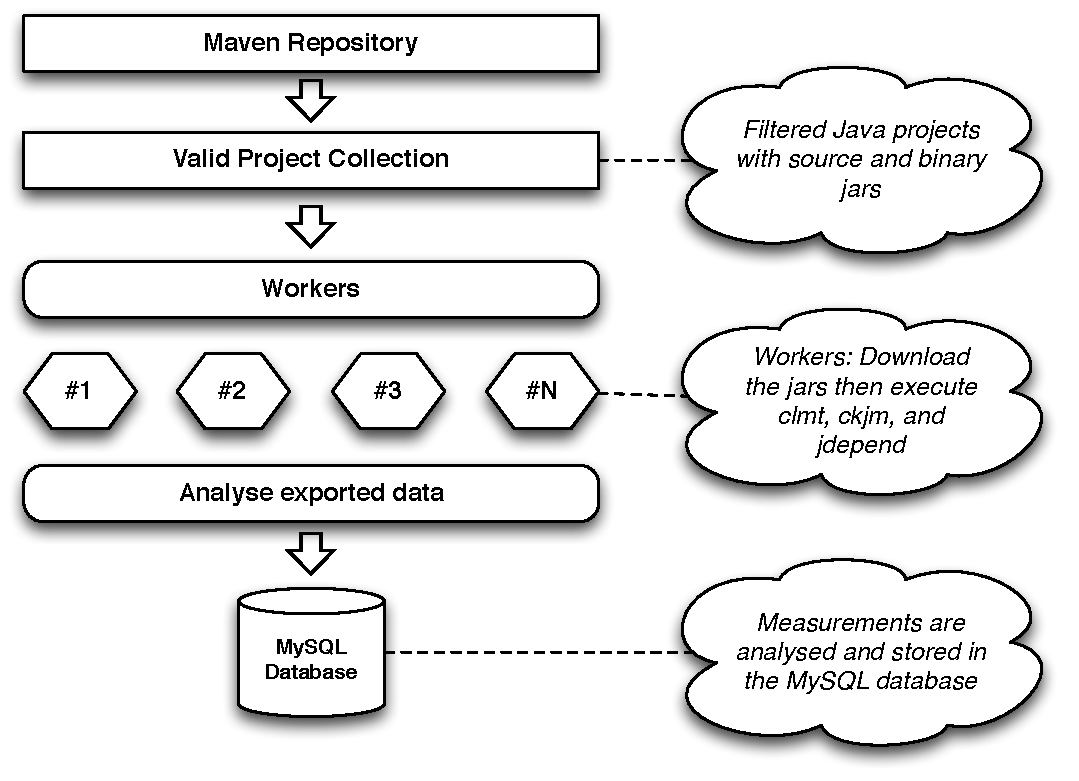
\includegraphics[scale=0.45]{import-process}
\caption{The dataset construction process.}
\label{fig:dataset-construction}
\end{figure}

The dataset construction process is illustrated in Figure~\ref{fig:dataset-construction}. In general, it follows the same methodology presented in reference \cite{MKLGS14}.

Initially, a snapshot of the Maven repository was downloaded locally. The repository contains various projects that contain several versions. In our experiment, we only used Java projects. For every Java project all versions were filtered out and only the latest was kept. The process to identify them was the following; Every project consists of two {\sc jar} files, one that contains a compiled version of the project and one that contains the source code. The projects that did not had both binary and source {\sc jar}s, were excluded from the experiment. When the source {\sc jar} file was downloaded, it was scanned for Java source files. If the source files were present in the archive, then the project was flagged as a valid Java project.

When the selection process was finished, we created a series of processing tasks based on the selected {\sc jar}s, and added them to a task queue mechanism. Then we executed a number of workers that checked out tasks from the queue, applied the static analysis tools on each {\sc jar} and stored the results to the data repository (a {\sc m}y{\sc sql} database system). The workers were written in Python. In addition, there were several shell scripts (bash) that performed several checks and sanitisation tasks (e.g. checking for malformed results). The tools that were applied on every {\sc jar} were the following:

\begin{itemize}
  \item \textbf{CKJM-ext} \textit{(ckjm)}~\cite{Spi05g}; which calculates many software metrics, including the \textit{Chidamber and Kemmerer} set of object-oriented metrics \cite{CHKE94}. The version of the tool that we used for this experiment can be found in GitHub~\cite{CKJM}.

  \item \textbf{JDepend} \textit{(jdep)}~\cite{JDEPEND}; a tool that analyses {\sc jar} files that contain compiled Java classes and calculates a series of design metrics.

  \item \textbf{CLMT} \textit{(clmt)}~\cite{SGKL09}; which stands for \textit{cross-language metric tool} and analyses the source code of several languages in order to calculate a series of size metrics.
\end{itemize}

\begin{table}[!t]
\centering
\caption{The selected Maven projects' size metrics.}
\label{tbl:oss-size-metrics}
\begin{tabular}{l r}
 \hline
\textbf{Metric} & \textbf{Value}\\
\hline
Project Count & 11,365\\
File Count & 449,213\\
Package Count & 59,436\\
Lines of Code & 74,565,772\\
Source Lines of Code & 40,921,287\\
Comment Lines of Code & 25,268,959\\
Number of Classes & 370,518\\
Number of Interfaces & 66,352\\
Number of Enumerations & 9,879\\
Measurement Count & 32,844,836\\
\hline
\end{tabular}
\end{table}

Table \ref{tbl:oss-size-metrics} presents several size metrics for our dataset. It includes 11,365 projects, with more than 74 million lines of code and almost 33 million unique measurements. Table~\ref{tbl:class-selected-metrics}, \ref{tbl:method-selected-metrics}, \ref{tbl:package-selected-metrics}, and \ref{tbl:size-selected-metrics} present the key metrics that are calculated and stored in the dataset. Each tool focuses on a different aspect of a software system; \textit{ckjm} focuses on object-oriented design metrics \cite{LOKI94}, \cite{CHKE94}, \textit{jdepend} on package design, while \textit{clmt} focuses on program size metrics. Several metrics are calculated by more than one tool, like \textit{cyclomatic complexity} \cite{cabe76}, which is calculated by both \textit{clmt} and \textit{ckjm}. Both calculations are available in the database.

A series of newly introduced metrics were also stored in the database. Such metrics can count the usage of specific {\sc dsl} application libraries in a software project and they are included in the Table~\ref{tbl:size-selected-metrics}. The methodology to identify and calculate the {\sc dsl} metrics was the following: A set of standard {\sc dsl} application libraries was identified, and the source was scanned for specific \textit{import} statements (e.g. \textit{java.util.regex}). These statements indicated that the standard package that implements regular expressions was used, thus regular expressions were used in the project. Build files or other resources that may contain {\sc dsl}s were not included. One final assumption was also made; if {\sc xp}ath or {\sc xslt} were found in the source code, then the project would be marked as a project that utilizes {\sc xml}. This is because both languages are used for query and transformations on {\sc xml} {\sc dom} trees. Table \ref{tbl:dsl-list} lists the selected {\sc dsl}s application libraries. Note that we focused on libraries that were included as part of the Java {\sc sdk}.

\begin{table}[!t]
\centering
\caption{List of selected {\sc dsl} application libraries.}
\label{tbl:dsl-list}
\begin{tabular}{l l}
 \hline
\textbf{DSL} & \textbf{Java Package}\\
\hline
Regular Expressions & \verb|java.util.regex|\\
XML & \verb|javax.xml|, \verb|org.w3c| and \verb|org.xml|\\
SQL & \verb|java.sql| and \verb|javax.sql|\\
XPath & \verb|java.xml.xpath|\\
XSLT & \verb|javax.xml.transform|\\
RTF & \verb|javax.swing.text.rtf|\\
HTML & \verb|javax.swing.text.html|\\
\hline
\end{tabular}
\end{table}

In Section~\ref{sec:dsl}, we describe an experiment based on these metrics. The experiment measures the popularity of {\sc dsl} usage for the dataset and therefore for the Java ecosystem in general.

\begin{table}[!t]
\centering
\caption{Class Design Metrics.}
\label{tbl:class-selected-metrics}
\begin{tabular}{l l}
\hline
Depth Of Inheritance Tree & \textit{ckjm}\\
Coupling Between Objects & \textit{ckjm}\\
Weighted Methods Per Class & \textit{ckjm}\\
Response For Class & \textit{ckjm}\\
Lack Of Cohesion In Methods & \textit{ckjm}\\
Number Of Children & \textit{ckjm}\\
Attribute Hiding Factor & \textit{clmt}\\
Coupling Between Methods & \textit{ckjm}\\
Average Method Complexity & \textit{ckjm}\\
Cohesion Among Methods of Class & \textit{ckjm}\\
Data Access Metric & \textit{ckjm, clmt}\\
Inheritance Coupling & \textit{ckjm}\\
Lack Of Cohesion In Methods3 & \textit{ckjm}\\
Measure Of Aggregation & \textit{ckjm}\\
Measure Of Functional Abstraction & \textit{ckjm}\\
Number of Attributes & \textit{clmt}\\
Method Hiding Factor & \textit{clmt}\\
\hline
\end{tabular}
\end{table}

\begin{table}[!t]
\centering
\caption{Method Design Metrics.}
\label{tbl:method-selected-metrics}
\begin{tabular}{l l}
\hline
Number of Method Parameters & \textit{clmt}\\
Number of Methods & \textit{clmt, ckjm}\\
McCabe Cyclomatic Complexity & \textit{ckjm, clmt}\\
\hline
\end{tabular}
\end{table}

\begin{table}[!t]
\centering
\caption{Package Design Metrics.}
\label{tbl:package-selected-metrics}
\begin{tabular}{l l}
\hline
Number of Concrete Classes & \textit{jdep}\\
Afferent Couplings & \textit{jdep, ckjm}\\
Efferent Couplings & \textit{jdep, ckjm}\\
Instability & \textit{jdep}\\
Abstractness & \textit{jdep}\\
Distance Main Sequence & \textit{jdep}\\
\hline
\end{tabular}
\end{table}

\begin{table}[!t]
\centering
\caption{Program Size Metrics.}
\label{tbl:size-selected-metrics}
\begin{tabular}{l l}
 \hline
Number of Classes & \textit{clmt, ckjm, jdep}\\
Number of Enumerations & \textit{clmt, ckjm}\\
Number of Interfaces & \textit{clmt, ckjm}\\
Module Count & \textit{clmt, ckjm}\\
Comments Lines Of Code & \textit{clmt}\\
Lines Of Code & \textit{clmt, ckjm}\\
Source Lines Of Code & \textit{clmt}\\
Function Oriented Code & \textit{clmt}\\
DSL Usage Count & \textit{clmt}\\
RTF Usage Count & \textit{clmt}\\
Regex Usage Count & \textit{clmt}\\
HTML Usage Count & \textit{clmt}\\
XPath Usage Count & \textit{clmt}\\
XSLT Usage Count & \textit{clmt}\\
XML Usage Count & \textit{clmt}\\
SQL Usage Count & \textit{clmt}\\
File Count & \textit{clmt}\\
\hline
\end{tabular}
\end{table}

\section{Database Structure}
\label{sec:db}

Figure~\ref{fig:database-schema} illustrates the database schema. Specifically, it consists of five tables; \textit{measurement}, \textit{category}, \textit{identifiers}, \textit{measurement\_type}, and \textit{project}. The central database table is \textit{measurement}, which holds the measurement values. The other tables can be used for normalization.

Metrics are divided into six categories that define their scope; \textit{module}, \textit{class}, \textit{method}, \textit{code unit}, and \textit{project-wide}. These values are stored in \textit{category} database table.

The descriptive names for each metric are stored in the \textit{measurement\_type} database table. There are 65 metrics available in the dataset. The names are composed by the actual metric name and the tool that was used to calculate them. For instance, \textit{McCabe\_clmt} denotes that the metric name is the McCabe cyclomatic complexity generated by the \textit{clmt} tool, while \textit{McCabe\_ckjm} means that it is the same metric calculated by the \textit{ckjm} tool.

Filenames, methods, classes and package names along with other identifiers are stored in the \textit{identifiers} table. Note that each measurement has a related filename and a related identifier that points to a software element. For example the \textit{afferent coupling} metric for the module in the directory ``com/scalagent/jmx'' is related to the identifier \textit{com.scalagent.jmx}.
Finally, the database table \textit{project} contains the related project identifiers, directly extracted from the maven repository.

\begin{figure*}
\centering
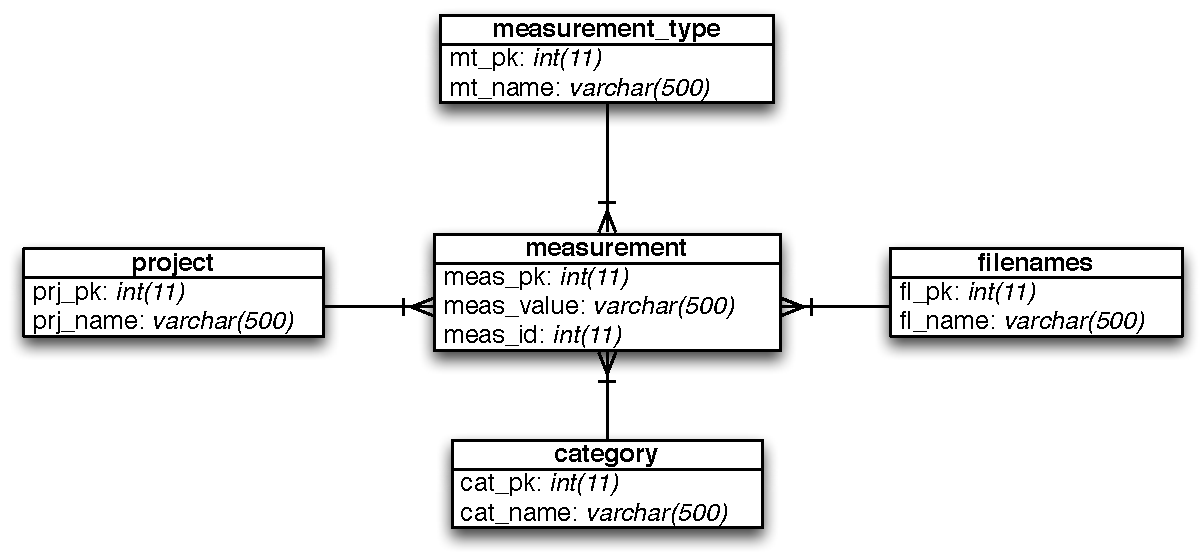
\includegraphics[scale=0.65]{database-schema}
\caption{The database schema.}
\label{fig:database-schema}
\end{figure*}

\section{Research Opportunities}
\label{sec:research-opportunities}

The measurements provided by our dataset, can be used by researchers and practitioners alike. Researchers can use the data to experiment with new software quality models, or validate them with real projects. Practitioners who develop tools that calculate metrics can use the dataset to validate if their tools produce correct results.

The dataset also includes the {\sc dsl}-related metrics, which quantifies the usage of basic {\sc dsl} application libraries that are already shipped with the Java {\sc sdk}. These kind of metrics, can be really useful for researchers that focus on {\sc dsl} embedding, or study {\sc dsl} usage patterns~\cite{KARA14} as we illustrate in the following section.

Finally, our dataset can be used side-by-side with the ones presented by Mitropoulos et al.~\cite{HP04} and Raemaekers et al.~\cite{RDV13} in order to examine the datasets for metric correlations. This is because their datasets were also produced by analyzing projects coming from the Maven repository.

\section{Experimenting with the Dataset}
\label{sec:dsl}

\begin{table}[!t]
\centering
\caption{Top {\sc dsl} Usage Combinations.}
\label{tbl:dsl-top-usage}
\begin{tabular}{l r}
 \hline
\textbf{DSLs} & \textbf{Count}\\
\hline
XML & 1,561\\
Regex & 909\\
SQL & 493\\
XML, XSLT & 475\\
Regex, XML, XSLT & 158\\
Regex, XML & 303\\
SQL, XML & 162\\
Regex, SQL & 116\\
Regex, SQL, XML, XSLT & 80\\
Regex, SQL, XML & 71\\
SQL, XML, XSLT & 54\\
XML, XPath & 50\\
\hline
\end{tabular}
\end{table}

The initial goal of this experiment was to provide quantifiable results that are indicative regarding the usage of {\sc dsl}s in multiple Java projects. The related metrics can be found in the database table named \textit{measuremnt\_type}, and they are the following: \textit{RTFUsage}, \textit{RegexUsage}, \textit{HTMLUsage}, \textit{HTMLUsage}, \textit{XPathUsage}, \textit{XSLTUsage}, \textit{XMLUsage}, \textit{SQLUsage}, and \textit{DSLCount}. A Python script that analysed the measurements stored in the database, we produced the results illustrated in Table~\ref{tbl:dsl-top-usage}. This table, lists popular {\sc dsl} usage combinations found in our dataset. An interesting observation is that {\sc xml} is the most widespread {\sc dsl} with 1,561 occurrences in 11,365 projects (13\%). Regular expressions are also popular with 909 occurrences (7\%). Note that the numbers represents the projects where {\sc xml} and regular expressions were used as the only {\sc dsl}.

\section{Limitations}
\label{sec:limit}

As we mentioned earlier, to produce our dataset we adopted a narrow selection process. In particular, we identified and analyzed only projects that were written in Java and had both the source code and the binary {\sc jar} available in the repository. The latter reduced significantly the number of projects that were analyzed, because many of them provided only the binary {\sc jar}. Since only \textit{clmt} analyses the source code, this resulted in the reduction of the number of measurements that exposed object-oriented and package design issues.

Finally, only one version was analyzed per project (the latest, unless it violated the aforementioned restriction).
This decision renders the dataset unusable, for research focused on software evolution.

\section{Related Work}
\label{sec:rel}

The Maven ecosystem has been previously analyzed by Raemaekers et al.~\cite{RDV13} to produce the {\it Maven dependency dataset}. Apart from basic information like individual methods, classes, packages and lines of code for every {\sc jar}, this dataset also includes a database with all the connections between the aforementioned elements.

Also, Mitropoulos et al. performed a similar experiment~\cite{MKLGS14}. In particular, they used the FindBugs~\cite{HP04} static analysis tool, to analyze a large part of the maven repository. Their dataset includes for each {\sc jar}, a corresponding bug collection produced by FindBugs. Our work differs from these two approaches since it presents the metrics calculated by the three different static analysis tools that calculate metrics regarding object-oriented design, program size, and package design.

\section{Conclusions}
\label{sec:conc}

We presented a dataset created by applying three different static analysis tools on Java projects coming from the Maven Central repository. The results invlove a variety of software metrics from program size to object-oriented design.
%In the future, we plan to keep an updated version of the dataset, by analysing the new additions and updates made in the repository.
We have also shown how our data can be used to extract meaningful results concerning {\sc dsl} usage in Java Projects.

As we discussed, our selection process was strict, filtering out projects that did not have the project's sources. However, we are planning to expand our project coverage in the future and include projects that cannot be analysed by all tools (due to source code unavailability).
Finally, by including all versions for each project we can allow researchers to use our dataset in the evolution context.

\section{Availability}

The dataset and the source code of this publication, along with some utility scripts are available at \url{https://github.com/bkarak/data_msr2015}. The {\sc sql} dump of the database is available at \url{http://gaijin.dmst.aueb.gr/~bkarak/data_msr2015.bz2}.

% use section* for acknowledgement
\section*{Acknowledgment}

%
%\begin{table}[!t]
%% increase table row spacing, adjust to taste
%\renewcommand{\arraystretch}{1.3}
% if using array.sty, it might be a good idea to tweak the value of
% \extrarowheight as needed to properly center the text within the cells
%\caption{An Example of a Table}
%\label{table_example}
%\centering
%% Some packages, such as MDW tools, offer better commands for making tables
%% than the plain LaTeX2e tabular which is used here.
%\begin{tabular}{|c||c|}
%\hline
%One & Two\\
%\hline
%Three & Four\\
%\hline
%\end{tabular}
%\end{table}






% trigger a \newpage just before the given reference
% number - used to balance the columns on the last page
% adjust value as needed - may need to be readjusted if
% the document is modified later
%\IEEEtriggeratref{8}
% The "triggered" command can be changed if desired:
%\IEEEtriggercmd{\enlargethispage{-5in}}

% references section

% can use a bibliography generated by BibTeX as a .bbl file
% BibTeX documentation can be easily obtained at:
% http://www.ctan.org/tex-archive/biblio/bibtex/contrib/doc/
% The IEEEtran BibTeX style support page is at:
% http://www.michaelshell.org/tex/ieeetran/bibtex/
\bibliographystyle{IEEEtran}
\bibliography{msr}

\end{document}


